\begin{figure}[ht]
    \centering
    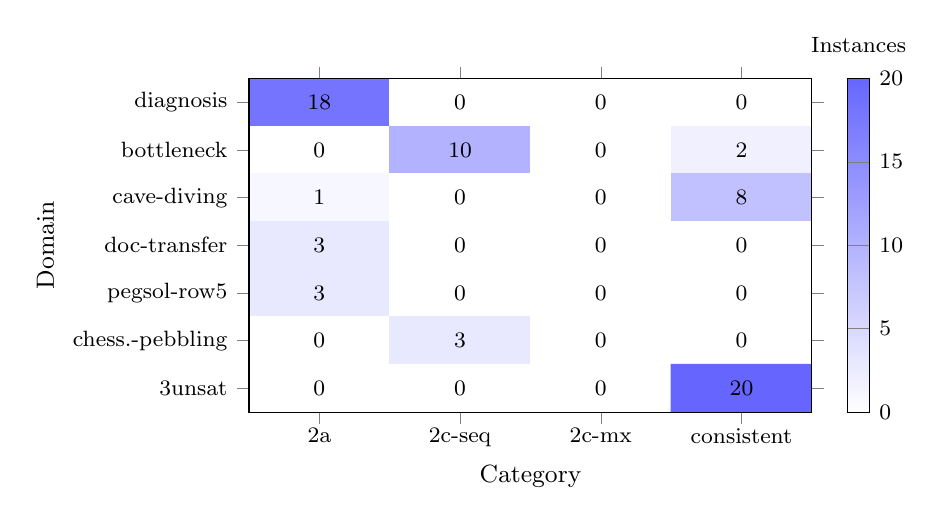
\begin{tikzpicture}
        \begin{axis}[
                width=0.72\textwidth,
                height=0.48\textwidth,
                enlargelimits=false,
                colormap={whiteblue}{color=(white) color=(blue!60)},
                colorbar,
                colorbar style={
                        width=8pt,
                        title={Instances},
                        title style={font=\footnotesize},
                        ytick={0,5,10,15,20},
                        tick label style={font=\footnotesize},
                    },
                point meta min=0,
                point meta max=20,
                xtick={0,1,2,3},
                xticklabels={2a, 2c-seq, 2c-mx, consistent},
                xticklabel style={font=\footnotesize},
                x tick label style={yshift=2pt},
                ytick={0,1,2,3,4,5,6},
                yticklabels={
                        diagnosis,
                        bottleneck,
                        cave-diving,
                        doc-transfer,
                        pegsol-row5,
                        chess.-pebbling,
                        3unsat},
                yticklabel style={font=\footnotesize},
                y dir=reverse,
                xlabel={Category},
                ylabel={Domain},
                label style={font=\small},
                tick align=outside,
                axis on top,
                nodes near coords,
                nodes near coords style={font=\footnotesize, anchor=center},
                every node near coord/.append style={
                        /pgf/number format/precision=0,
                        /pgf/number format/fixed,
                    },
            ]
            \addplot[
                matrix plot,
                mesh/cols=4,
                point meta=explicit,
                nodes near coords={\pgfmathprintnumber\pgfplotspointmeta},
            ] table[meta=C] {
                    x y C
                    0 0 18
                    1 0 0
                    2 0 0
                    3 0 0
                    0 1 0
                    1 1 10
                    2 1 0
                    3 1 2
                    0 2 1
                    1 2 0
                    2 2 0
                    3 2 8
                    0 3 3
                    1 3 0
                    2 3 0
                    3 3 0
                    0 4 3
                    1 4 0
                    2 4 0
                    3 4 0
                    0 5 0
                    1 5 3
                    2 5 0
                    3 5 0
                    0 6 0
                    1 6 0
                    2 6 0
                    3 6 20
                };
        \end{axis}
    \end{tikzpicture}
    \caption{Category classifications per domain across the 68 computed unsolvable instances.}
    \label{fig:category_distribution}
\end{figure}
